 %Linea Para poder completar automaticamente las citas con el Sublime
%No hace el documento, se puede borrar esta linea si no se usa el Sublime
%------------------------------------------------------------------------------
 \newcommand{\NoBiblioIntro}[1]{
 \ifthenelse{\equal{#1}{verdadero}}{}{\bibliography{Referencias/base_bibliografica}}
 \NoBiblioIntro{verdadero}}
 %-----------------------------------------------------------------------------

%Formato (Nombre de capitulo largo o corto), nombre del capitulo y estilo de la
%Portada del Capitulo
%------------------------------------------------------------------------------

 %Formato en si, titulo en un solo renglon
 \FormatoCapituloUnaLinea

 %Nombre y etiquete para referir
 \chapter{Introducción}\label{chap:Introduccion}
 %\label{chap:Introduccion}

 %Para que no salga el numero de pagina en la portada del capitulo
 \thispagestyle{empty}
	
 %Resumen del Capitulo en Italica
 \noindent\textit{la Intro}

 
 %Indice de capitulo alineada al borde inferior de la pagina, nueva pagina
 \vfill
 \minitoc
 \newpage
 %-------------------------------------------------------------------------------

\section{Breve reseña sobre nanotecnología}

	En su conferencia, \textit{<<There's Plenty of Room at the Bottom>>} del 29 de diciembre de 1959, el físico Richard Feynman, considerado por muchos el padre de la nanotecnología, sugirió que se podría escribir toda la enciclopedia británica en la cabeza de un alfiler.\cite{Feynman1959} Esta presentación fue sin duda más conceptual e inspiradora que estrictamente científica, anterior al uso masivo de las técnicas de microscopia electrónica y al desarrollo de las microscopias de efecto túnel y fuerza atómica. Pocos años después se publica la fabricación del primer transistor (de varios centímetros cúbicos), el cuál que estaba muy lejos de convertirse en la unidad básica del cálculo computacional que es hoy en día, de unas pocas decenas de nanométros cuadrados. 

	Años más tarde Taniguchi incorpora por primera vez el termino nanotecnología para describir procesos de microfabricación como deposito de películas delgadas o \textit{ion millling} y lo define como <<aquellos procesos de separación, consolidación y deformación de los materiales átomo por átomo o molécula por molécula>>. \cite{taniguchi1974} Fue Drexler quien finalmente popularizó el termino en su libro \textit{<<Engines of Creation: The Coming Era of Nanotechnology>>}\cite{drexler1987}. 

	Una definición más actual y consensuada para nanotecnología puede ser: desarrollo tecnológico de estructuras y sistemas en una escala nanométrica (entre 1 y \SI{100}{\nm}). Se podría, también, establecer una definición funcional: uso e implementación tecnológica de nanociencia. Esta rama de la ciencia se caracteriza fundamentalmente por ser multidisciplinaria y abarcar muchas áreas del conocimiento, ciencia de materiales, química, física y biología (por citar algunas) las cuales interactúan entre sí para generar un espacio sinérgico entre ellas. Cuando los descubrimientos en nanociencia son potencialmente aplicables a productos interviene la nanotecnología, tendiendo un lazo entre la ciencia y la industria para llevar a cabo desarrollos tecnológicos o escalar prototipos que eventualmente puedan acabar en productos de consumo.
	
	Al realizar una búsqueda en la base de datos Scopus\textsuperscript\textregistered (\url{http://www.scopus.com}) de las publicaciones que contienen las palabras en ingles para nanotecnología (\textit{nanotechnology}), nanofísica (\textit{nanophysics}), nanoquímica (\textit{nanochemistry}), nanoescala (\textit{nanoscale}) y nanociencia (\textit{nanoscience}) se obtienen los resultados de la figura \ref{fig:publicaciones-ano}. 

		%Grafico de los paises
			\vspace*{-0.7cm}
 			\begin{figure}[ht!]
 			\begin{center}
 			\includegraphics[width=0.74\textwidth]{Graficos/busqueda-por-ano.pdf}
 			\vspace*{-0.4cm}
 			\caption[Publicaciones por año en nanotecnología]{Publicaciones científicas por año que contienen la palabra \textit{nanotechnology}, \textit{nanoscale}, \textit{nanoscience}, \textit{nanochemistry} o \textit{nanophysics} en el título, resumen o palabras claves.}
 			\label{fig:publicaciones-ano} 		    
 			\end{center}
 		    \end{figure}
	
	Del análisis de dicho gráficos se observa que las publicaciones que contiene la palabra nanotecnología en el título, resumen o como palabra clave son mucho mayor que las que contiene nanoescala, nanociencia, nanofísica o nanoquímica. Contrariamente a la evolución histórica de las ``ciencia aplicadas'', donde primero es el descubrimiento científico y luego el desarrollo tecnológico, la nanotecnología parece presentarse como impulsora, no solo de desarrollos tecnológicos sino también como impulsora de ``ciencias básicas''.

	Whiteside y Deutch en su articulo \textit{<<Let's practical>>} opinan que la química, como rama de la ciencia básica y como industria madura, debe reinventarse para acondicionarse a los requerimientos de la sociedad actual y poder seguir respondiendo preguntas fundamentales a la vez que resuelve problemas del mundo real, los autores afirman que que los ``problemas prácticos'' son generalmente despreciados por las ciencias básicas. \cite{Burdass2010} Sin embargo este no parece ser el caso de la nanotecnología que a hecho grandes contribuciones al desarrollo científico a pesar de ser una disciplina que en general busca resolver problemas prácticos.
	
	Este hecho se ve reflejado si se agrupan los resultados de la búsqueda de la figura \ref{fig:publicaciones-ano} por países, vemos que aquellos que más publicaciones tienen con la palabra nanotecnología, son, como es de esperable los países mas desarrollados tecnológicamente, ocupando los primeros cinco lugares, Estados Unidos, China, Japón, Alemania y Reino Unido. En América Latina, el primero es Brasil con 1453 publicaciones seguido de Argentina, con 567 (figura \ref{fig:paises}).

			\begin{figure}[ht!]
 				\begin{center}
 				\includegraphics[angle=270,width=0.75\textwidth]{Graficos/histogramas-ciencia.pdf}
 				\caption[Nanotecnología por países]{Distribución por países del numero de publicaciones científicas con la palabra nanotecnología. Datos obtenidos de la base de datos Scopus.}
 				\label{fig:paises}
 		    	\end{center}
 		    	\end{figure}

	Además de producción científica y desarrollos tecnológicos, la nanotecnología cuenta patentes internacionales y productos industriales de consumo masivo en el mercado global. Existen bases de datos que registran la actividad del sector creando informes sobre estos productos, patentes, estándares y compañías con base nanotecnologica. Podemos mencionar algunas de ellas como el \textit{Nanotechnology Consumer Products Inventory} (CPI) (\url{http://www.nanotechproject.org/cpi/}) creada por \textit{The Project on Emerging Nanotechnologies} en 2005\cite{Vance2015}; la \textit{Nanotechnology Products Database} (NPD) (\url{http://http://product.statnano.com/}) creada con apoyo del \textit{Iran Nanotechnology Initiative Council} (INIC) en 2010 y \textit{The Nanodatabase} (\url{http://nanodb.dk}) iniciativa desarrollada por \textit{DTU Environment, Danish Ecological Council} y \textit{Danish Consumer Council} en 2011. En el gráfico de la figura \ref{fig:productos} se resumen algunos datos registrados en cada una de ellas, agrupados por cantidad productos con base nanotecnologica, numero de empresas que los generan y cantidad países donde se encuentran distribuidas.

		\begin{figure}[ht!]
 			\begin{center}
 			\includegraphics[angle=270,width=0.80\textwidth]{Graficos/productos2.pdf}
 			\caption[Cantidad de productos, compañías y origen con base nanotecnologica]{Registros de empresas y paises generadores de producto que incorporan nanotecnología. Extraido de las bases de datos \textit{Nanotechnology Consumer Products Inventory} (CPI), \textit{Nanotechnology Products Database} (NPD) y \textit{The Nanodatabase}.}
 			\label{fig:productos}
 		    \end{center}
 		    \end{figure}

 	También existen numerosas patentes que registran productos con nanotecnología. En la figura \ref{fig:patentes} se muestra la evolución desde el año 2001 hasta el 2016 del numero de patentes registradas por la \textit{European Patent Office} (EPO) y por la \textit{United States Patent and Trademark Office} (USPTO).

		\begin{figure}[ht!]
 			\begin{center}
 			\includegraphics[width=0.75\textwidth]{Graficos/patentes.pdf}
 			\caption[Numero de patentes de productos en base nanotecnologica]{Numero de patentes registradas por año en la oficinas de patentes de los Estados Unidos y Europa. Datos extraídos de \url{http://statnano.com/}.}
 			\label{fig:patentes}
 		    \end{center}
 		    \end{figure}

 	Mucho de estos productos pertenecen al rubro alimenticio y cosmético. Nanopartículas de Ag, TiO$_2$ o SiO$_2$ se incorporan en los alimentos o en los envases como conservantes, agentes antimicrobianos, colorantes y antioxidantes. En la industria cosmética el mayor uso de las nanomateriales es para dar color, textura y como filtros solares.
 	La inclusión de nanomateriales en el mercado, especialmente en estos dos rubros, obliga la incorporación de recomendaciones, estandarización y regulaciones en el campo de la nanotecnología.  El documento CEN/TC 352 (\url{https://standards.cen.eu/dyn/www/f?p=204:32:0::::FSP_ORG_ID,FSP_LANG_ID:508478,25&cs=18E152154F73BA190A16C4D279047F5FD}) del \textit{European committee for Standardization} (CEN) ofrece guías para la identificación, detección y cuantificación de nano-objetos en matrices complejas. La \textit{International Organization for Standardization} (ISO) publicó una serie de documentos ISO/TC 223 (\url{https://www.iso.org/committee/381983.html}) con el objetivo de definir y establecer el alcance de las nanotecnologías. Define allí una serie de parámetros y descriptores para caracterizar e identificar nanoparticulas, tamaño, forma, distribución, composición química, carga superficial, estado de agregación, solubilidad y área especifica entre otros.

 	Este contexto de regulaciones emergentes en el campo de la nanotectnología obliga a los institutos metrologicos de los distintos países (entre ellos el INTI, como Instituto Metrológico Nacional) a generar nanomateriales de referencia y validar las técnicas y procedimientos para su detección y cuantificación.

 	Hasta el momentos se ha hecho una breve introducción sobre la historia y situación actual de la nanotecnología, pero ¿como se construyen los nanomateriales?.

	Existen dos enfoques posibles para obtener estructuras y objetos en la nanoescala. El primero se trata de realizar estructuras por grabado o maquinado de un material, para llevarlo a las dimensiones nano. Esta aproximación se denomina de <<arriba hacía abajo>> o más conocida como \textit{top-down}. Desde la invención del transistor en 1948 las técnicas de miniaturización \textit{top-down} no pararon de multiplicarse y llegar a dimensión realmente asombrosas como los transistores actuales con canales de \SI{10}{nm}. Pertenecen a este grupo las técnicas de fotolitografía, grabado por vía húmeda o seca y gran parte de la tecnología del silicio se basa en esta aproximación (es decir toda la electrónica actual de consumo masivo incluyendo computadoras y dispositivos móviles). 

	El segundo enfoque es aquel denominado de <<abajo hacía arriba>> o \textit{bottom-up} el cual consiste en la construcción de objetos a partir de bloques fundamentales, los cuales pueden ser átomos o moléculas. La nanotecnología se caracteriza por aprovechar propiedades diferentes del material volumétrico que surgen en esta escala. La mayoría de estos descubrimientos, cambios ópticos, eléctricos, magnéticos o mecánicos se deben a al enfoque \textit{bottom-up}, así como nuevas formar de sintetizar materiales, p. ej. grafeno, nanotubos de carbono o fullerenos. Faraday fue uno de los primeros científicos en sugerir que, en la escala nanométrica, el cambio en las propiedades de la materia está ligado al tamaño, estudiando el cambio de color en coloides de Au\cite{faraday1857}. A este grupo pertenecen las técnicas químicas de síntesis de nanopartículas, nanobarras y películas delgadas, métodos de autoensamblado y química supramolecular; también técnicas de crecimiento en fase vapor: epitaxial, \textit{physical vapour deposition (PVD)}, \textit{chemical vapour deposition} (CVD) y \textit{atomic layer deposition (ALD)}.
			
	Es de esperar que la verdadera revolución nanotecnologica de un salto de calidad cuando converjan ambos enfoques. Las técnicas ya industrializadas de miniaturización aprovechando las propiedades de diferenciales y novedosas. Este se trata de un enfoque ``funcional'', en el cual lo importate es el objetivo, ya sea un trabajo científico, prototipo o un producto.

	Soler-Illia expone en su libro <<Nanotecnología: el desafío del siglo XXI>>\cite{nanotecnologia-galo} que es en este periodo de la historia donde se esta llevando a cabo esta convergencia. A modo de ejemplo presentan un gráfico esquemático donde muestra la evolución de ambos enfoques hacia la convergencia en la nanoescala.

			\begin{figure}[ht!]
 				\begin{center}
 				\includegraphics[width=0.75\textwidth]{Imagenes/convergencia2.png}
 				\caption[Convergencia \textit{top-down }y \textit{bottom-up.}]{Convergencia temporal de las aproximaciones \textit{top-down }y \textit{bottom-up.} Figura extraída de <<Nanotecnología: El desafío del siglo XXI>>.}
 				\label{fig:galo-convergencia}
 		   	    \end{center}
 		   	    \end{figure}

    Esta tesis tiene por objetivo fabricar sensores utilizando electroquímica como técnica de detección. La fabricación de los mismos se realiza en base a procesos \textit{top-down} para escalar y miniturizar los electrodos y procesos \textit{bottom-up} (quimica sol-gel y autoensamblado inducido por evaporación) con el fin sintetizar la película activa. El diagrama de  de Venn de la figura \ref{fig:sensores} muestran los elementos necesarios para la fabricación de los sensores electroquímicos basados en películas delgadas mesoporosas. 
	
	       \begin{figure}[ht!]
 				\begin{center}
 				\includegraphics[width=0.60\textwidth]{Esquemas/concepto-interdiplinario.pdf}
 				\caption[Plataforma de sensores. Diagrama de Venn.]{Elementos necesarios para el desarrollo y fabricación de la plataforma de sensores electroquímicos basados en películas delgadas mesoporosas.}
 		   		\label{fig:sensores}
 		    	\end{center}
 		    	\end{figure}
 	
 	En las secciones secciones se tratan brevemente los fundamentos teóricos de cada una de las áreas temáticas exploradas para el desarrollos de la plataforma de sensores electroquímicos en base a películas delgadas mesoporosas y hacía el final del capítulo se exponen los objetivos y motivaciones que llevaron a materializar esta tesis.

\section{Películas delgadas mesoporosas}\label{sec:mesoporosos}
	
	El termino película delgada o lamina delgadas hace referencia a una capa de material cuyo espesor que va desde unos pocos manómetros a algunos micrones, típicamente entre 10 y \SI{1000}{\nm}. El control en el espesor de la película es una etapa fundamental para cualquier aplicación, mas aun cuando se trata de controlar la propiedades que surgen debido a la dimensión nanométrica en el espesor (p. ej. fenómenos de interferencia de luz en el rango visible con espesores entre 400 y \SI{750}{\nm}). 
    Las peliculas delgadas son elaboradas a partir de técnicas químicas que utilizan precursores moleculares, comúnmente conocidas como procesos \textit{bottom-up}. Dentro de ellos se pueden nombrar los procesos de autoensamblado molecular, electrodeposición, crecimiento epitaxial, técnicas de deposición químicas o físicas en fase vapor, sol-gel y autoensamblado inducido por evaporación entre las más populares. En particular las películas delgadas mesoporosas (\pdm) son aquellas que además de la característica de ser delgadas, son porosas, con arreglos de poros ordenados a largo o corto alcance.

	La \textit{International Union of Pure and Applied Chemistry} (IUPAC) definen los materiales mesoporosos como aquellos que presentan poros monodispersos entre 2 y \SI{50}{\nm}. La porosidad es una medida de los espacios vacíos (poros) en un material, es una fracción del volumen de poros sobre el volumen total, entre 0 y 1 (o entre 0\% y 100\%).\cite{iupac-1994} Confiere a los materiales importantes propiedades, como una baja densidad lo que supone un peso ligero y gran área superficial para almacenar moléculas en los poros. Además, el tamaño del poro puede funcionar como un tamiz para separar moléculas de distintos tamaños.\cite{Martin2004} 

	La producción de óxidos mesoporosos (ya sean polvos, películas o xeorgeles) se realiza a través de la combinación precursores inorgánicos y de compuestos poliméricos para formar los poros. Involucra dos procesos concertados: la formación y el autoensamblado de micelas, molde de la estructura de poros, y las reacciones químicas de hidrólisis y condensación del precursor inorgánico que formará el óxido. 

				\begin{figure}[h!]
 				\begin{center}
 				\includegraphics[width=\textwidth]{Esquemas/oxido-meso.pdf}
 				\caption[Esquema general para la formación de un óxido mesoestructurado]{Esquema general para la formación de un óxido mesoestructurado combinando química sol-gel y autoensamblado inducido por evaporación (AEIE).}
 		   		\label{fig:oxmeso}
 		    	\end{center}
 		    	\end{figure}

	\pagebreak En la Figura \ref{fig:oxmeso} se muestra un esquema de los pasos involucrados en la obtención de óxidos mesoporosos. En una primera etapa se forma un sistema híbrido orgánico-inorgánico que contiene al surfactante rodeado por el óxido (sistema mesoestructurado). En un segundo paso, se elimina el surfactante dando lugar a la estructura porosa. La eliminación del surfactante puede ser por calcinación o extracción.

	%Los óxidos mesoporosos se obtienen a partir de la formación del óxido en presencia de un agente moldeante. En estas síntesis se combinan dos técnicas: las reacciones de tipo sol- gel y el autoensamblado de surfactantes. La primera, mediante el control de la hidrolisis y condensación del precursor inorgánico, da lugar al óxido y la segunda, a partir de la formación de micelas, forma el molde del arreglo poroso14,15 .
    %La síntesis de óxidos mesoporosos se puede resumir como se muestra la Figura 2. 
		 

    El primer antecedente de una síntesis de sílice mesoporosas se registra en una patente del año 1971. Sin embargo el campo de los materiales mesoporosos comenzó a desarrollarse de manera explosiva a partir del trabajo del grupo de Mobil. Científicos de esta firma reportaron en 1992 la síntesis en polvo de la familia de sílices mesoporosas conocida como M41S (MCM-41, MCM-48, etc.). Entre 1997 y 1998 se reportan los primeros trabajos en los cuales de obtuvieron óxidos de silicio mesoporoso en forma de película delgada mediante técnicas de evaporación controlada y \textit{dip-coating}.\cite{Lu1997,Zhao1998a,Zhao1998,Brinker1999} 

    A partir de estos trabajos pioneros el numero de publicaciones sobre potenciales aplicaciones y usos creció considerablemente, reportándose síntesis para óxidos de metales de transición \cite{Ciesla1996,Ulagappan1996,Antonelli1995}, óxidos híbridos, poros de una gran variedad de tamaños, estructuras porosas jerárquicas, etc.\cite{Soler-Illia2006,Moller1998} %CITAS

   
	% 1) mesoporoso

	% 2) eq

	% 3) microfa

	% Citas:

	% 1) de complejo a ser algo sencillo \\
	% 2) trabajo en INTI, aplicado....
	% 3) Nanotecnologia.... combiancaion microfab con sol-gel... tema central
	% 4) conjunto interseccion entre las 3 patas, EQ, microfab y sol-gel


	% 			El porque se elijo oxido de silicio, porque F127.... muy importante!
				
	% 			Esta etapa del trabajo involucró la síntesis por sol-gel de películas delgadas de óxido de silicio mesoporoso. La película de oxido es la base de cual partimos para construir la <<palicula activa>>, es por ello que es de suma importancia escoger los elementos fundacionales de esta película. \cite{Soler-Illia2002a,Brinker1999,Soler-Illia2006,Grosso2004,Innocenzi2013}

	% 			\begin{enumerate}
	% 				\item El óxido que define las propiedades estructurales (Morfología, cristalinidad, espesor), ópticas y eléctricas.
	% 				\item El tamaño, estructura y caracteristicas de los poros.
	% 			\end{enumerate}

	% 			Vamos a repasar porque elegimos el óxido de silicio, y no otros oxido de metales tales como Ti, Zr, Al, los cuales se han demostrado que son propicios para hacer estructuras mesoporoosas. El SiO$_2$ es aislante eléctrico y no absorbe en el rango UV/VIS. Estas dos características son fundamentales para los sensores, si bien la primera es común a la mayoritaria de los óxidos de transición, algunos de ellos presentan propiedades de semiconductores, 

	% 			Descripcion de como se sintetizan las peliculas, preparacion de los soles, porque no se usa CTAB ni brij, ni Titanio oxido (quimica del silicio mas rica, mas economica, no absorbe en el UV/VSI)

	% 			Descripcion de Spin - Coating (una sola cara, facilmente escalable, integrable a la industria microelectronica, ventajas de utilizar spin en lugar de dip, (pero tambien se puede utilizar dip, sobre todo para piezas no planas y de mayor volumen)

	% 			Proceso de calcinacion. Despoito sobre Au, Vidrio y Solicio.

	% 			Porque: gran area superficial, escablables, bajos costos, tuneable como filtro por tamaño de poro, quimicamente facil de modicar la superfie, optica adsocion en el UV (por esto no se puede de Ti02, pero si de ZrO4) despoitable por inkjet\cite{Lian2013,Mougenot2006a}, spin (microelectronica), dip (superficies de dificil geometria.)
	% 			Aplicaciones en microfluidica \cite{schmuhl2005,Martinez2009}
				
	% \subsection{sol-gel}	



	
	%La Real Academia Español tiene tres acepciones para la palabra <<poro>>. Dos se ellas son <<Espacio que hay entre las moléculas de los cuerpos>> y <<Intersticio que hay entre las partículas de los sólidos de estructura discontinua>> (\url{http://dle.rae.es/?id=ThdH0Y9%7CThe6N27%7CThgVys6}). Según esta definición todos los materiales presentan poros (excepto por supuesto los átomos o moléculas individuales, pero estos no entran dentro de la definición de material), resulta indispensable cuantificar la porosidad o la cantidad de poros en un material. La porosidad es una medida de espacios vacíos en un material, es una fracción del volumen de poros sobre el volumen total, entre 0 y 1 (o entre 0\% y 100\%).\cite{iupac-1994} Confiere a los materiales importantes propiedades, como una baja densidad lo que supone un peso ligero y gran área superficial para almacenar moléculas en los poros. Además, el tamaño del poro puede funcionar como un tamiz para separar moléculas.\cite{Martin2004} 

	%La \textit{International Union of Pure and Applied Chemistry} (IUPAC) divide a los materiales porosos en tres según el tamaño de poro. Los materiales microporosos, con poros de menos de \SI{2}{\nm} de diámetros, los mesoporosos con poros entre 2 y \SI{50}{\nm} y los macroporosos con poros de diámetro mayores a \SI{50}{\nm}.\cite{iupac-1994}

	%Entre 1997 y 1998 se reportan los primeros trabajos en los cuales de obtuvieron óxidos de silicio mesoporoso en forma de película delgada mediante técnicas de evaporación controlada y \textit{dip-coating}.\cite{Lu1997,Zhao1998a,Zhao1998,Brinker1999} A partir de estos trabajos el numero de publicaciones sobre potenciales aplicaciones y usos creció considerablemente, reportándose síntesis para óxidos de metales de transición puros o combinados \cite{Ciesla1996,Ulagappan1996,Antonelli1995}, óxidos híbridos, poros de una gran variedad de tamaños, estructuras porosas jerarquicas, etc.\cite{Soler-Illia2006,Moller1998} %CITAS

	\subsection{Química sol-gel}

	Los procesos tipo sol-gel refieren a una síntesis inorgánica en la cual se parte un precursor molecular en suspensión coloidal (sol) y, mediante reacciones de hidrólisis y de condensación, se  forma una estructura inorgánica tipo gel o densa del material deseado. Dependiendo de procesamiento del sol se pueden obtener distintas formas de la materia según las aplicaciones o los usos para los cuales se quieran emplearla los productos de la síntesis. Entre ellas se cuentan: fibras, nanoparticulas, polvos, películas delgadas densas o porosas, arogeles y xerogeles por citar los mas utilizados.

	El control sobre las cinéticas de tales reacciones permite disponer de formas y estructuras diferentes, tanto en cuanto a la cristalinidad como a la porosidad del cerámico resultante. Las temperaturas involucradas en la síntesis sol-gel son muy inferiores ($\leq$\SI{400}{\celsius}) a la de los métodos tradicionales utilizados para la fabricación de materiales cerámico ($\geq$\SI{700}{\celsius}).\cite{Brinker1990,Jolivet2000,Wright2001}

	La formación de un óxido por el método sol-gel implica conectar centros metálicos mediante puentes oxo o hidroxo para generar (hidroxo)polímeros de metal en solución. Para ello se hace reaccionar un precursor MX$_4$ con agua, donde M es el elemento del cual se quiere obtener el óxido y X es un anión inorgánico o un grupo –OR. El primer paso de la reacción es la hidrólisis de un grupo alcóxido (o de un anión) para dar lugar a un hidroxocompuesto, tal como se ejemplifica en la ecuación \ref{eq:hidrosg1} para el caso de un alcóxido.
			
			 \begin{equation}
 				\begin{aligned}
 				\includegraphics[scale=0.70]{Esquemas/sg1.pdf}
 				\end{aligned}
 				\label{eq:hidrosg1}
 	 			\end{equation}

	Luego, la especie hidroxilada puede reaccionar con otros centros metálicos, dando lugar a reacciones de condensación, cuyos productos son oligómeros y, eventualmente, partículas de óxido. La condensación puede dar lugar a un puente oxo, tal como se muestra en la ecuación \ref{eq:oxosg2} (oxolación) o un puente hidroxo, tal como se observa en \ref{eq:olasg3} (olación). 

			\begin{equation}
		    	\begin{aligned}
 	 	 		\includegraphics[width=0.9\textwidth]{Esquemas/sg2.pdf}
 	 	 		\end{aligned}
 	 	 		\label{eq:oxosg2}
 	 	 		\end{equation}

			\begin{equation}
 	 	 		\begin{aligned}
 	 	 		\includegraphics[width=0.9\textwidth]{Esquemas/sg3.pdf}
 	 	 		\label{eq:olasg3}
 	 	 		\end{aligned}
 	 	 		\end{equation}

	La hidrólisis y la condensación son los equivalentes a la activación y la propagación en la polimerización orgánica, por lo que el proceso sol-gel puede calificarse como una polimerización inorgánica controlada. Un manejo adecuado de las variables (concentración de precursores, catalizadores, pH, solvente) y condiciones de síntesis (temperatura, humedad, tiempos de cada etapa de reacción) lleva a sistemas donde se pueden controlar con precisión  la estructura cristalina, el arreglo de los poros, la incorporación de funciones orgánicas, la relación en óxidos de mixtos (MM') y demás características del sistema.

	Para profundizar sobre estos temas se recomienda la lectura de los libros <<Sol Gel Science. The Physics and Chemistry of Sol Gel Processing>>\cite{Wright2001} o <<Introduction to Sol Gel Processing>>. \cite{Pierre1998} 

	%Los materiales usados para hacer películas delgadas pueden ser de origen orgánicos, inorgánicos e híbridos. Los más utilizados son los inorgánicos, y dentro de este grupo los metálicos y cerámicos.
	
	
	

	\subsection{Autoensamblado inducido por evaporación (AEIE)}

	El proceso de Autoensamblado inducido por evaporación (AEIE) fue introducido por por el grupo de Brinker a fines de la década de 1990.\cite{Lu1997,Brinker1999} Consiste en la formación de estructuras supramoleculares de surfactantes, obtenidas por la evaporación del solvente en el que el polímero se halla inicialmente disuelto. Este proceso ocurre cooperativamente con la interacción y condensación de los precursores inorgánicos. En la actualidad, este concepto constituye un método habitual de obtención de \pdm\space ordenadas\cite{Grosso2004} así como micropartículas, monolitos, etc.\cite{Yang1998a}

	Existente muchas técnicas para obtener \pdm\space, las más utilizadas son \textit{spin-coating}, \textit{dip-coating} y \textit{spray-coating}. En la figura \ref{fig:autoensam} se ejemplifica el proceso de AEIE cuando se aplica la técnica de \textit{dip-coting}. Allí se destacan los principales eventos que ocurren al retirar el sustrato de la solución a velocidad controlada. El sol, en términos generales, está compuesto por un solvente volátil, precursores inorgánicos, agua y el surfactante deseado. A medida que se retira el sustrato, se evapora el solvente y consecuentemente se concentra el surfactante mas allá de la concentración micelar critica (cmc), formando micelas, que luego se organizarán en un cristal líquido. La estructura de dicho cristal precede impacta directamente en la estructura final de las \pdm. Procesos similares ocurren cuando se obtienen \pdm\space por \textit{spin-coating}. 
 			
 			\begin{figure}[th!]
 				\begin{center}
 				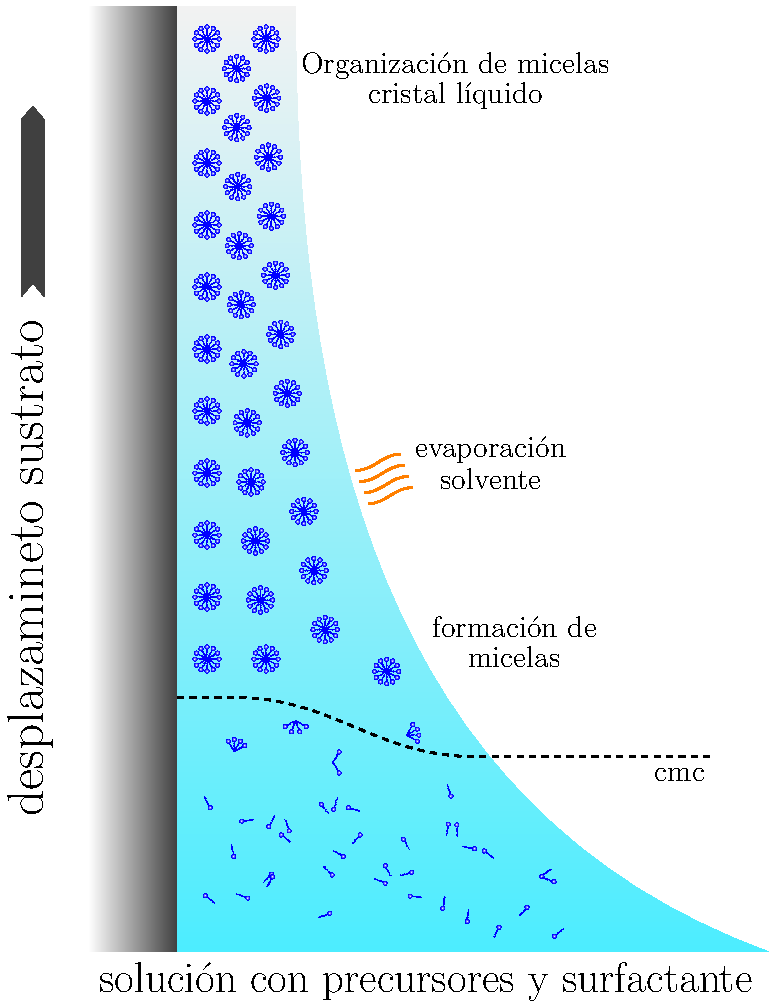
\includegraphics[width=0.5\textwidth]{Esquemas/autoensam.pdf}
 				\caption[Proceso de autoensamblado inducido por evaporación (AEIE)]{Proceso de autoensamblado inducido por evaporación (AEIE) mediante \textit{dip-coating}. La evaporación del solvente favorece la formación de micelas mas allá de la cmc formado el cristal líquido. Un proceso similar ocurre cuando se aplica la técnica de \textit{spin-coating}}
 		   		\label{fig:autoensam}
 		    	\end{center}
 		    	\end{figure}
	
   	En función de la composición inicial del sol, del tipo de surfactante, de la química de los precursores, del sustrato y de las condiciones ambientales es posible obtener diferentes condiciones que darán lugar a distintos arreglos tridimensionales de poros, que está dado por el organización micelar previo al momento en el cual se elimina el surfactante ya sea por calcinación o extracción.\cite{Grosso2004,Grosso2002,Crepaldi2002a,Grosso2003,Violi2015} 
	



	%\subsection{Aplicaciones}
		%“Los materiales porosos pueden servir como anfitriones de catalizadores o como vehículos para transportar fármacos y realizar una liberación controlada de moléculas específicas”, señala la investigadora. La porosidad también es útil para modificar las propiedades intrínsecas de los materiales.
	 	
	 	%En concreto, el grupo de investigación de Paula Ferreira desarrolla materiales porosos en diversas formas y composiciones y destinados a diferentes aplicaciones. “Realizamos materiales porosos híbridos en los que integramos moléculas orgánicas con óxido de silicio para capturar y separar gases”, comenta, así como “catálisis heterogénea y adsorción de contaminantes en el agua”.
		%Usos comerciales y en que formas, NP, materiales, sectores de aplicaciones. Low K.

\section{Electroquímica en películas delgadas mesoporosas}
	
\section{Miniaturización y escalabilidad}\label{sec:microfabricacion}\label{sec:intro_fotolito}
	
		%\subsection{microfabricacion}

		%\subsection{Litografia}

		%\subsection{Desposito}

		La industria de los semiconductores es hoy en día una de las más grandes y rentables del mundo, productora de computadoras, celulares, tabletas, etc. Una de las claves del continuo crecimiento de esta industria durante las ultimas 40 años fue el desarrollo del procesamiento del silicio y la tecnología planar. Los transistores se basa en proceso difusivos de impurezas dentro del silicio y la tecnología planar es el apilamiento sobre la oblea de silicio sucesivos de películas delgadas metálicas y  películas delgadas dieléctricas para contactar los transistores y hacer las pistas del circuito integrados. 

% %``''Todo deberia hacerse tan simple como sea posible, pero no mas que eso``'' Einsten.

% %\url{https://www.ted.com/talks/george_whitesides_toward_a_science_of_simplicity?language=es}\cite{ted_whitesides2010}
% Portabilidad

% \section{Microfabricacion}\label{sec:microfabricacion}

% Porque se elijio Au, Electroquimica, etc.

% Sputt: explicar sputt, fotolito porque microelectronica, MEMS, sensores.
% En los casos que se depositó la capa dieléctrica de SiO$_2$ se hizo con la fuente de radiofrecuencia (RF), mientras que los depósitos de las películas metálicas se realizaron con la fuente de corriente directa (DC), ambas configuradass a potencia constante, a P=\SI{400}{\watt}.  De esta forma se deja libre la tensión y la corriente, parámeros que dependen a su vez del vacío en la cámara, de la distancia entre el cátodo y el ánodo y el caudal de argón.\cite{sigmund1968}. 

% \subsection{Fotolitografia}\label{sec:intro_fotolito}

% \subsection{sputtering}

% \section{implementacion tecnologica}
% nanotecnologia\cite{Gimenez2017}
% Intergrar bottom-up, top-down y hacer un dispositivo intergrado, miniaturizado, escalado, industrializable, tecnologicamente compatible, IC, logica, sensores MEM
% Integracion, todo en argentina, valor agregado del proceso sol-gel.\cite{Volksen2010}

% \section{Aplicaciones}

\section{Motivaciones y objetivos}

	El presente trabajo de tesis se desarrolló en el Instituto Nacional de Tecnología Industrial (INTI), cuyas principales actividades son: certificación de productos, metrología industrial, científica y legal, y generación y transferencia	de innovación tecnológica a la industria. Es, dentro de este contexto, que surge el desafío de desarrollar un dispositivo en base nanotecnologica con posibilidad de ser transferido . 

	El objetivo principal de la tesis es desarrollar una plataforma de sensores electroquímicos basados en películas delgadas mesoporosas. Las etapas y objetivos intermedios para la fabricación de los sensores se pueden resumir en los siguientes items:

	\begin{itemize}
		
		\item Depositar y condensar películas delgadas mesoporosas de óxidos de silicio estructuradas con F127 y CTAB sobre silicio, películas delgadas de oro y microelectrodos.  
		
		\item Desarrollar métodos para condensar la estructura inorgánica (óxidos de silicio y silicio/circonio) y extraer el agente moldeante a temperaturas menores a los \SI{150}{\celsius}, de forma de evitar temperaturas de calcinación. 

		\item Compatibilizar procesos de síntesis \textit{bottom-up} con técnicas de microfabricación tipo \textit{top-down}. Mejorar adherencia, minimizar procesos difusivos y evitar condiciones agresivas de condensación.

		\item Estudio de propiedades de transporte, calculo de parámetros característicos mediante experimentos de electroquímica y simulación computacional por métodos de elementos finitos.

		\item Miniaturizacion de los sensores, estudios de escalabilidad, optimización de los diseños y pruebas electroquímicas funcionales.

		\end{itemize}	

	Finalmente cabe destacar, que este proyecto tiene por propósito, a mediano/largo plazo, fabricar una plataforma de sensores analiticos selectivos incorporando nanotecnología, portable, integrable en circuitos integrados, de bajo costo y con posibilidades de ser transferido a la industria.